\chapter{Material e M�todos ou Desenvolvimento do Projeto}
\label{Material}


% % % % % % % % % % % % % % % % % % % % % % % % % % % % % % % % % % % % % % % % % % % % % % % % % % %
\section{Material}



% % % % % % % % % % % % % % % % % % % % % % % % % % % % % % % % % % % % % % % % % % % % % % % % % % %
\section{M�todos}

\par A metodologia utilizada para realizar este trabalho baseia-se nas metodologias utilizadas em~\cite{Barros},~\cite{Yeo} e~\cite{Chen}. Basicamente o processo se divide conforme mostra a figura~\ref{fig:processo}.

\begin{figure}[H]
	\centering
	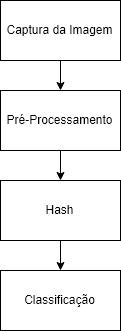
\includegraphics[width=0.2\textwidth]{./Resources/procedimento.png}
	\caption{M�todo utilizado.}
	\label{fig:processo}
\end{figure}

\subsection{Captura da Imagem}

\par A captura da imagem � feita pela c�mera do aparelho Android. N�o foi imposta nenhuma restri��o quanto �s caracter�sticas da c�mera para este projeto.

\subsection{Pr�-Processamento}

\par O pr�-processamento � realizado com aux�lio da biblioteca \textit{OpenCV} e consiste em tratar a imagem capturada pela c�mera de modo isolar as caracter�sticas desejadas (neste caso, busca-se isolar a regi�o das m�os).

\par O processo de pr�-processamento � mostrado na figura~\ref{fig:pre_proc}. S�o realizadas 3 etapas de maneira independente:

\begin{itemize}
	\item Detec��o de bordas: feita por meio da fun��o \textit{Imgproc.Canny}. 
	\item Detec��o de face: utiliza o \textit{CascadeClassifier} da biblioteca \textit{OpenCV} para fazer a detec��o da regi�o quadrada que cont�m uma face. Esta regi�o � ent�o preenchida (preto) de modo a eliminar a face da imagem.
	\item Detec��o de pele: 
\end{itemize}

\begin{figure}[H]
	\centering
	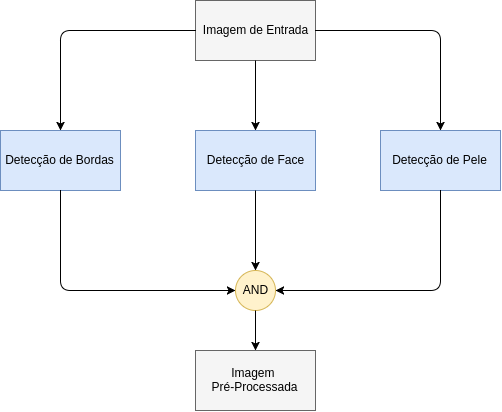
\includegraphics[width=0.7\textwidth]{./Resources/pre_processamento.png}
	\caption{Pr�-Processamento aplicado.}
	\label{fig:pre_proc}
\end{figure}

